\documentclass[11pt,a4paper]{ctexart}
\usepackage[margin=2cm]{geometry}
\usepackage{amsmath,amssymb,bm}
\usepackage{booktabs,graphicx,xcolor,hyperref,array,float}
\hypersetup{colorlinks=true,linkcolor=blue,urlcolor=blue}
\setlength{\parindent}{2em}
\setlength{\parskip}{0.25em}
\title{IMU--UWB InEKF：Task04 位姿传播公式改进}
\author{作者冻结姿态近似与 $J_l/Q_l$ 精确积分的受控对照}
\date{2026年7月27日}

\begin{document}
\pagestyle{plain}
\maketitle

\section{任务范围}

本任务从论文作者原始提交
\begin{center}
\texttt{f3b664e0e8c86b62c6ed2ea2a112261810228e1c}
\end{center}
独立导出代码到
\begin{center}
\texttt{imu-uwb-inekf-update-improve}
\end{center}
唯一被修改的作者跟踪文件是
\texttt{scripts/estimation/inekf.py}，且只改变名义速度和位置的 IMU 积分项。
旋转传播、协方差传播、UWB 量测、NIS 门限、状态注入、偏置、噪声和地面约束均
保持作者实现原样；作者论文与代码中的其他已知不一致也没有在本任务中顺带修复。

\section{论文原式：冻结步首姿态}

令偏置补偿后的角速度和比力为
\begin{equation}
 \omega_k=\omega_{m,k}-\hat b_{g,k},\qquad
 a_k=a_{m,k}-\hat b_{a,k}.
\end{equation}
Oursland 与 Mehrabian 原论文式 (39) 及作者代码采用
\begin{align}
 \hat R_{k+1}
 &=\hat R_k\exp\!\left((\omega_k\Delta t)^\wedge\right),\\
 \hat v_{k+1}
 &=\hat v_k+\left(\hat R_k a_k+g\right)\Delta t,\\
 \hat p_{k+1}
 &=\hat p_k+\hat v_k\Delta t
 +\frac12\left(\hat R_k a_k+g\right)\Delta t^2.
 \label{eq:author}
\end{align}
虽然旋转本身使用指数映射，平移项却在整个采样间隔内冻结
$\hat R(t)\approx\hat R_k$。因此式 \eqref{eq:author} 等价于把旋转中比力积分的
一阶、二阶矩阵函数分别近似为 $I$ 和 $\tfrac12I$。

\section{改进式：分段常值 IMU 下的精确积分}

在一个采样间隔内假定 $\omega_k,a_k$ 为常数。对
$0\leq\tau\leq\Delta t$，
\begin{equation}
 \hat R(t_k+\tau)
 =\hat R_k\exp(\omega_k^\wedge\tau).
\end{equation}
定义
\begin{equation}
 \phi_k=\omega_k\Delta t,\qquad
 \theta_k=\|\phi_k\|,\qquad
 \Phi_k=\phi_k^\wedge .
\end{equation}
参考文献 \texttt{eq\_ob.pdf} 给出的第一、第二阶左雅可比为
\begin{align}
 J_l(\phi)
 &=I+\frac{1-\cos\theta}{\theta^2}\Phi
 +\frac{\theta-\sin\theta}{\theta^3}\Phi^2,\\
 Q_l(\phi)
 &=\frac12I+\frac{\theta-\sin\theta}{\theta^3}\Phi
 +\frac{\theta^2+2\cos\theta-2}{2\theta^4}\Phi^2.
\end{align}
它们满足
\begin{align}
 \int_0^{\Delta t}\exp(\omega^\wedge\tau)\,d\tau
 &=J_l(\omega\Delta t)\Delta t,\\
 \int_0^{\Delta t}\int_0^u
 \exp(\omega^\wedge\tau)\,d\tau\,du
 &=Q_l(\omega\Delta t)\Delta t^2.
\end{align}
由此得到本任务使用的位姿传播：
\begin{equation}
\boxed{
\begin{aligned}
 \hat R_{k+1}
 &=\hat R_k\exp(\Phi_k),\\
 \hat v_{k+1}
 &=\hat v_k+g\Delta t
 +\hat R_kJ_l(\phi_k)a_k\Delta t,\\
 \hat p_{k+1}
 &=\hat p_k+\hat v_k\Delta t+\frac12g\Delta t^2
 +\hat R_kQ_l(\phi_k)a_k\Delta t^2.
\end{aligned}}
\label{eq:improved}
\end{equation}

\subsection{与原式的严格关系及数值实现}

小角度级数为
\begin{align}
 J_l(\phi)
 &=I+\frac12\Phi+\frac16\Phi^2+\mathcal O(\|\phi\|^3),\\
 Q_l(\phi)
 &=\frac12I+\frac16\Phi+\frac1{24}\Phi^2
 +\mathcal O(\|\phi\|^3).
\end{align}
因此作者原式就是 $J_l\approx I,\ Q_l\approx\tfrac12I$ 的截断；
当 $\omega_k=0$ 时，改进式又严格退化为作者原式。实现对
$\|\phi\|<10^{-4}$ 的三角系数采用泰勒级数，避免
$1-\cos\theta$ 和 $\theta-\sin\theta$ 的消减误差，而不是改变数学模型。

\section{代码映射与自动验证}

在 \texttt{InEKF.predict} 内，原代码
\begin{equation}
 R_ka_k\Delta t,\qquad
 \frac12R_ka_k\Delta t^2
\end{equation}
分别替换为
\begin{equation}
 R_kJ_l(\phi_k)a_k\Delta t,\qquad
 R_kQ_l(\phi_k)a_k\Delta t^2.
\end{equation}
辅助函数 \texttt{SO3\_motion\_jacobians} 同时计算两个矩阵，从而共享
$\Phi,\Phi^2,\theta^2$。自动测试共 $4/4$ 通过：
\begin{enumerate}
 \item 五组零角、小角、一般角和大角输入下，$J_l/Q_l$ 与 $9\times9$
 增广矩阵指数的对应块在 $2\times10^{-12}$ 容差内一致；
 \item 恒定角速度和比力的单步状态与闭式真值达到机器精度，作者冻结姿态式产生
 可检测的速度和位置截断误差；
 \item 零角速度时，改进状态与作者状态在 $10^{-14}$ 绝对容差内一致；
 \item 作者备份提交和全部原跟踪文件均受范围检查保护，除
 \texttt{inekf.py} 外没有原文件变化。
\end{enumerate}

\section{数据集配对结果}

比较入口向两种公式提供相同初值、时间戳、IMU、UWB、协方差和门限逻辑。
指标使用全部回放状态；姿态采用 $SO(3)$ 测地角，而不是旋转向量分量差。

\begin{table}[H]
\centering
\small
\caption{const1-trial1-tdoa2，前 30 s，30,267 次预测和 14,289 次 UWB}
\begin{tabular}{lrrr}
\toprule
指标 & 作者冻结姿态 & 改进 $J_l/Q_l$ & 相对变化\\
\midrule
位置 RMSE / m & 0.113244377 & 0.113243527 & $-0.000750\%$\\
速度 RMSE / (m/s) & 0.067806094 & 0.067795289 & $-0.015936\%$\\
姿态测地 RMSE / rad & 0.053281483 & 0.053245049 & $-0.068381\%$\\
yaw RMSE / rad & 0.051465742 & 0.051427884 & $-0.073561\%$\\
UWB 拒绝数 & 0 & 0 & 不变\\
\bottomrule
\end{tabular}
\end{table}

\begin{table}[H]
\centering
\small
\caption{const4-trial7-tdoa2-manual1，前 60 s，60,531 次预测和 25,915 次 UWB}
\begin{tabular}{lrrr}
\toprule
指标 & 作者冻结姿态 & 改进 $J_l/Q_l$ & 相对变化\\
\midrule
位置 RMSE / m & 0.355254510 & 0.355251628 & $-0.000811\%$\\
速度 RMSE / (m/s) & 0.187816636 & 0.187748699 & $-0.036172\%$\\
姿态测地 RMSE / rad & 0.103965884 & 0.103938205 & $-0.026623\%$\\
yaw RMSE / rad & 0.093971539 & 0.093941190 & $-0.032295\%$\\
UWB 拒绝数 & 138 & 138 & 不变\\
\bottomrule
\end{tabular}
\end{table}

const1 和 const4 的最大前后位置状态差分别为
$1.47\times10^{-4}$ m 和 $4.97\times10^{-4}$ m，最大速度状态差分别为
$1.14\times10^{-3}$ m/s 和 $1.55\times10^{-3}$ m/s。量级很小但非零，
符合约 1 kHz IMU 下高阶旋转积分修正的预期。两组四项 RMSE 均小幅改善，
但只依据两组数据不能宣称在所有轨迹上必然提高精度。

\clearpage
\begin{figure}[H]
\centering
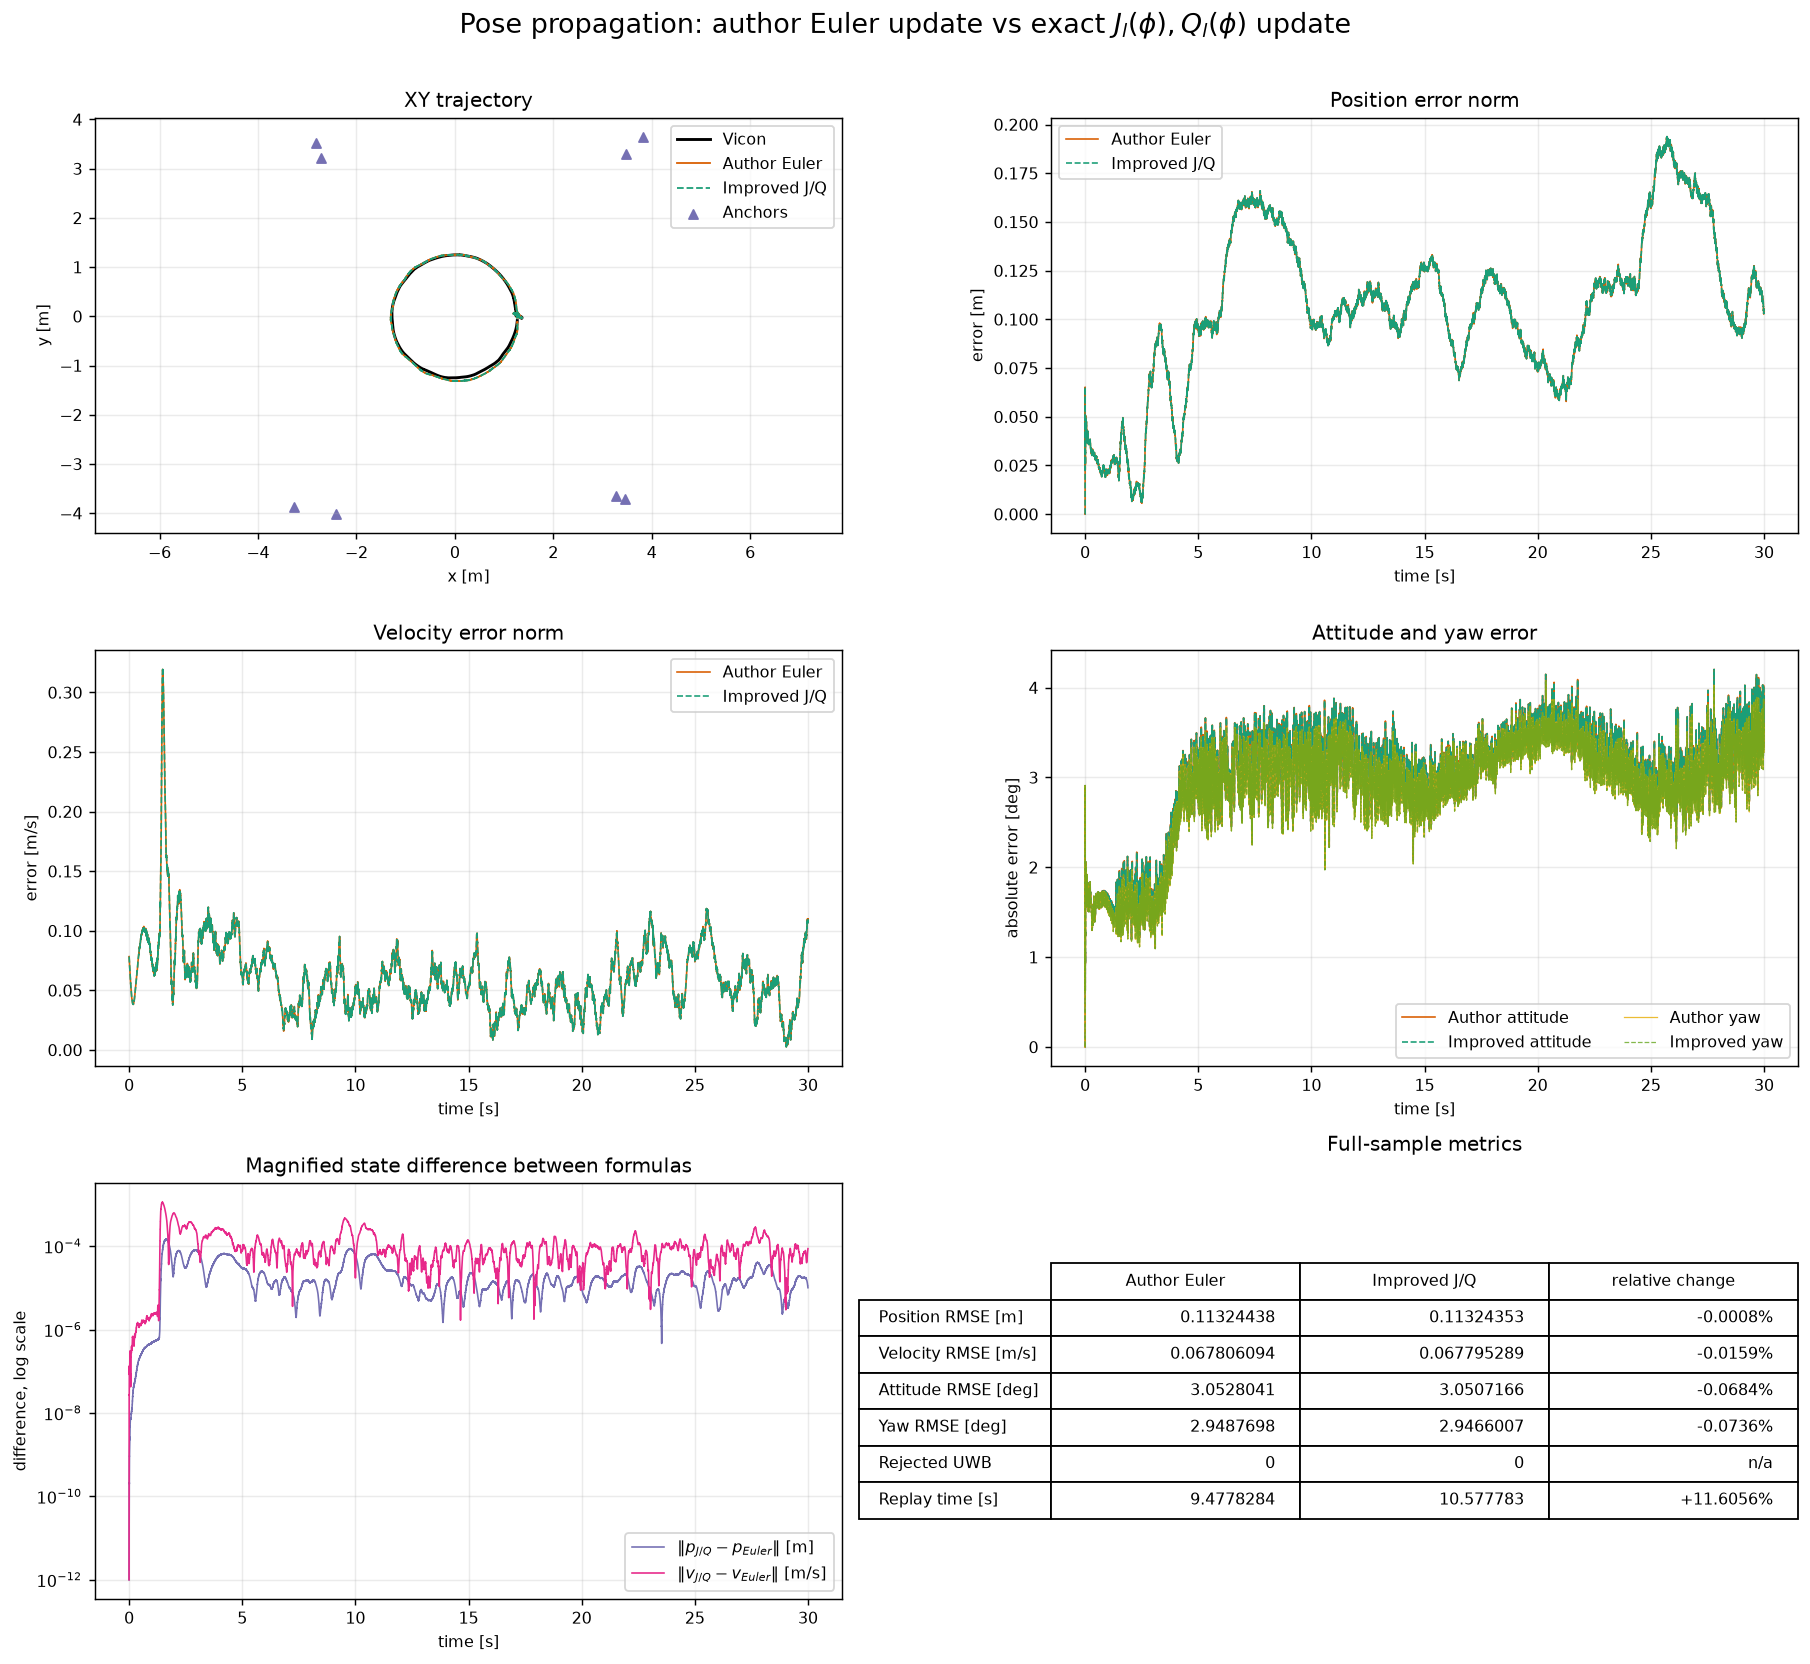
\includegraphics[width=\textwidth]{../imu-uwb-inekf-update-improve/results/task04_const1_30s/comparison.png}
\caption{const1 前 30 s 对比。轨迹和误差连续，主曲线近乎重合；左下对数图放大了
两种传播公式导致的状态差。}
\end{figure}

\clearpage
\begin{figure}[H]
\centering
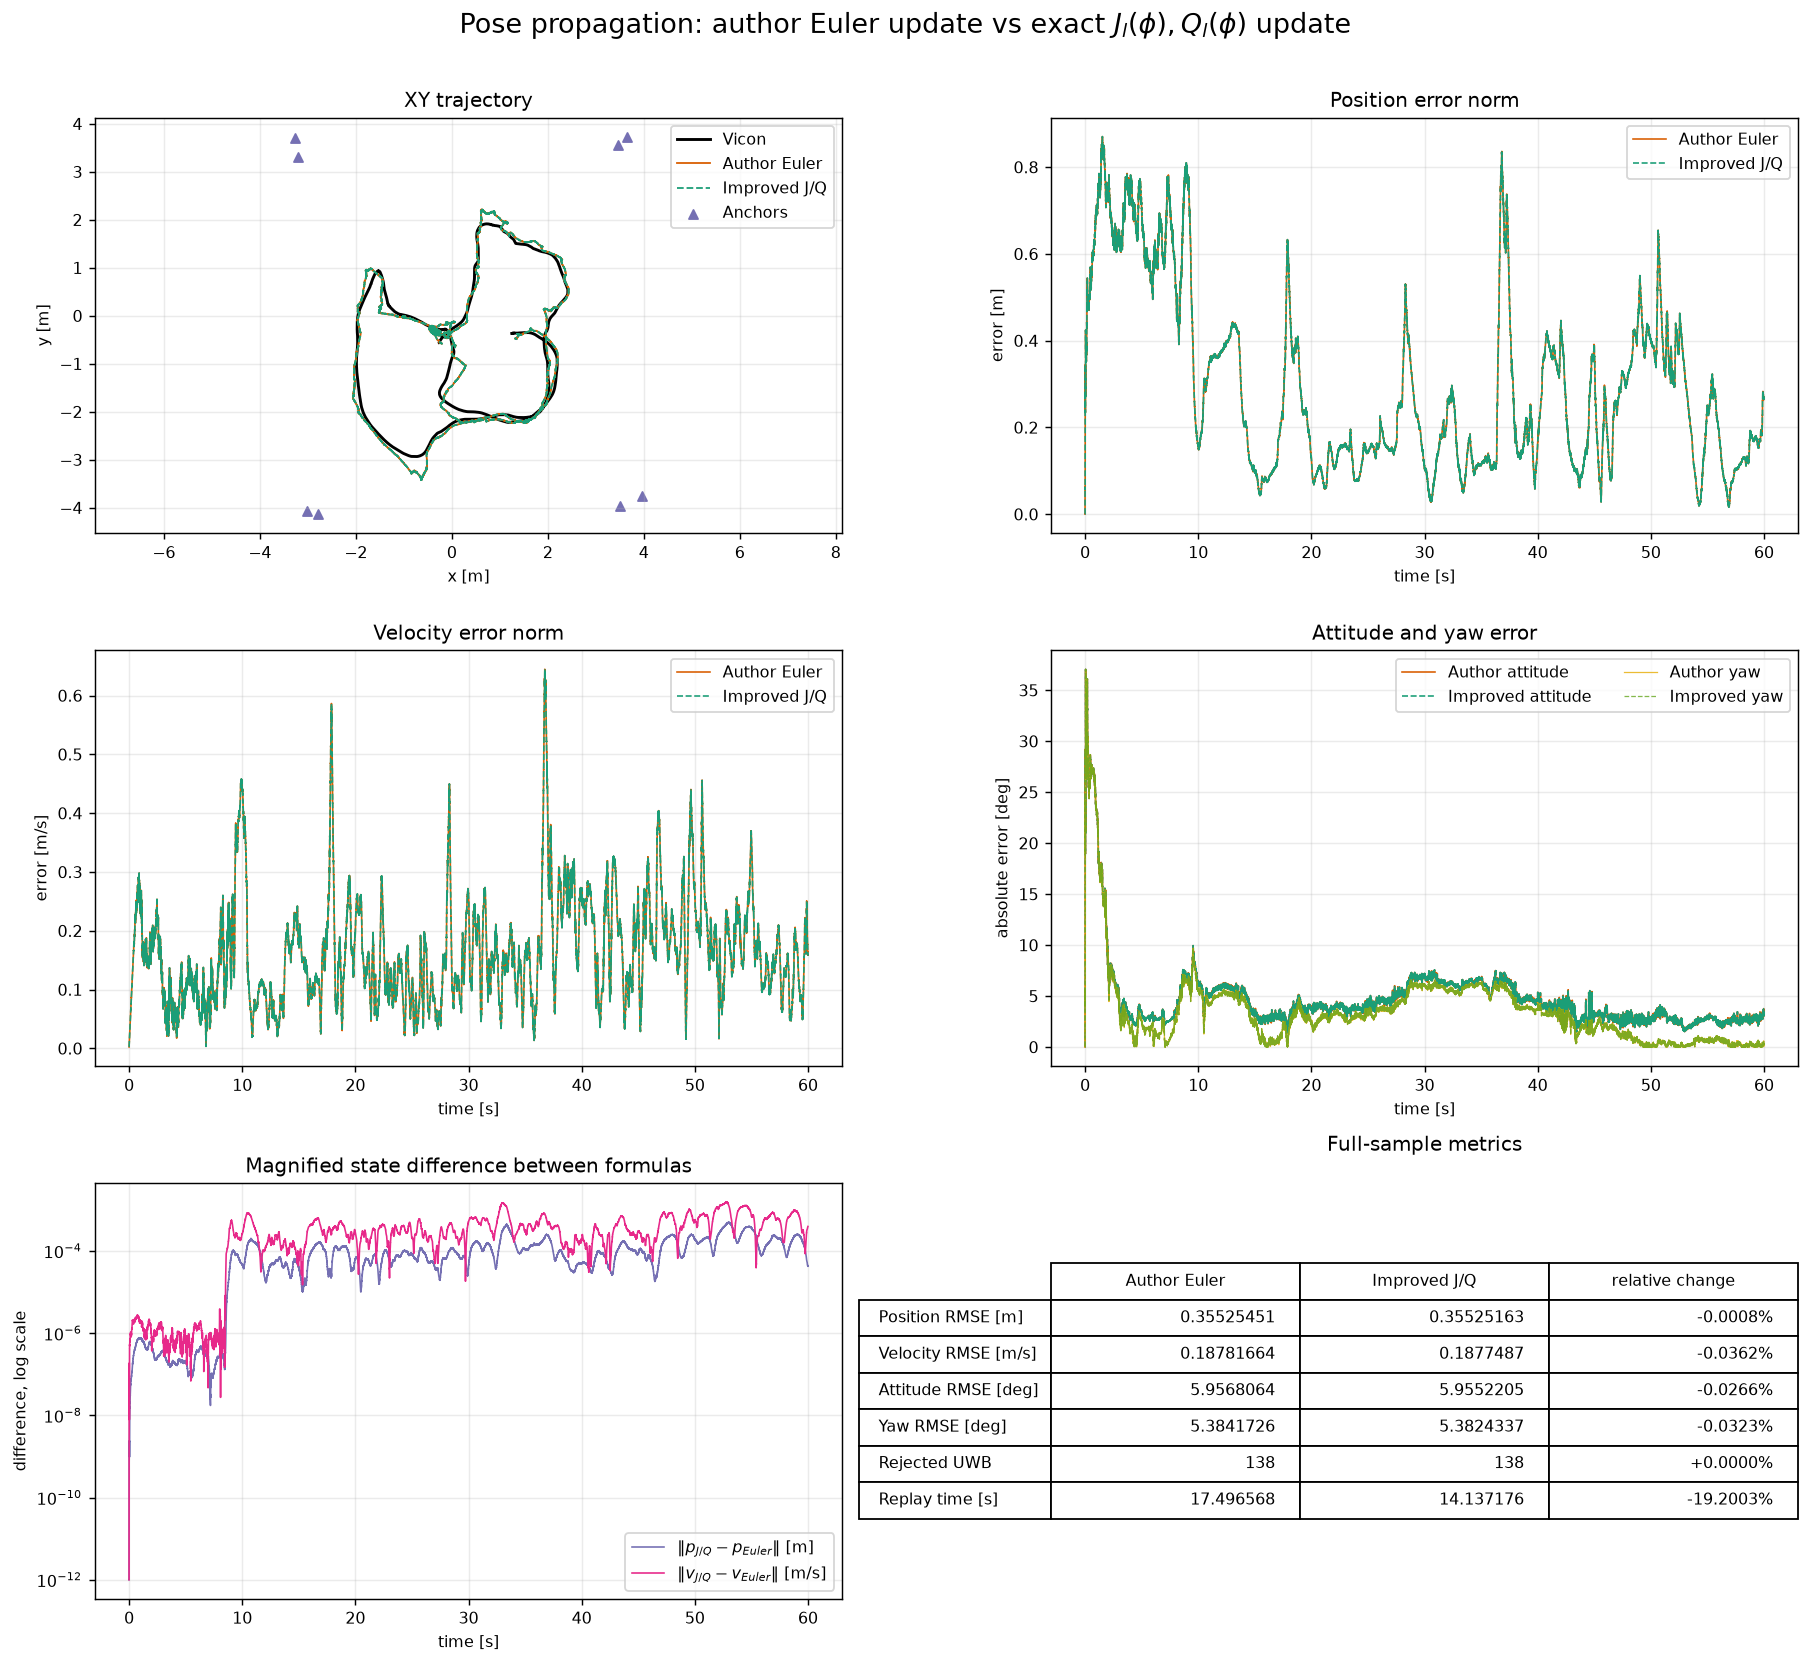
\includegraphics[width=\textwidth]{../imu-uwb-inekf-update-improve/results/task04_const4_manual1_60s/comparison.png}
\caption{const4 手动转动前 60 s 对比。没有新增跳变或发散，UWB 拒绝数保持
138；更强转动下的状态公式差异比 const1 更明显。}
\end{figure}

\clearpage
\section{计算开销估算与 AB/BA 验证}

\subsection{相对作者公式的新增工作}

共同的旋转更新 $R_{k+1}=R_k\exp(\phi_k^\wedge)$ 不重复计入。当前
\texttt{J\_l/Q\_l} 实现在一般角度分支中相对作者平移式增加
\begin{equation}
\boxed{
\begin{aligned}
 &3\text{ 次 }3\times3\text{ 矩阵乘法},\\
 &\text{约 }129\text{ 次标量乘法}+92\text{ 次标量加法},\\
 &1\text{ 次 sqrt}+1\text{ 次 sin}+2\text{ 次 cos},
\end{aligned}}
\end{equation}
以及少量标量除法和 NumPy 临时对象。小角泰勒分支保留矩阵运算，但不调用辅助
$\sqrt{\cdot}$、$\sin$、$\cos$。滤波状态、协方差和历史维度不变，持久内存增量
为零；四个显式 $3\times3$ \texttt{float64} 临时矩阵的纯数据载荷共
$4\times9\times8=288$ B。

\subsection{微基准与完整回放}

基准固定数值库单线程。两个角度分支各交替预热 3 s，再执行 9 轮局部公式微基准；
const1 和 const4 的 5 s 片段各执行 8 轮 AB/BA 完整回放。计时包含预测、15 维
协方差、UWB 更新和相同历史复制，排除数据加载、滤波器构造、指标和绘图。

\begin{table}[H]
\centering
\small
\caption{公式局部成本，中位数和 MAD}
\begin{tabular}{lrrrr}
\toprule
分支 & 作者/us & 改进/us & ratio 开销 & 配对开销中位\\
\midrule
一般角度 & 41.581 & 57.333 & $+37.884\%$ & $+38.453\%$\\
小角泰勒 & 41.009 & 57.181 & $+39.436\%$ & $+37.974\%$\\
\bottomrule
\end{tabular}
\end{table}

局部公式绝对增加约 $15.8$--$16.2~\mu$s/预测。完整滤波中，协方差传播、UWB
更新和历史仍占主要成本，因此总体比例明显降低：

\begin{table}[H]
\centering
\small
\caption{完整 InEKF 的 8 轮 AB/BA 回放}
\begin{tabular}{lrrrrr}
\toprule
数据 & 预测/UWB & 作者/s & 改进/s & ratio 开销 & 配对中位\\
\midrule
const1 5 s & 5044/2365 & 1.607188 & 1.693794 & $+5.389\%$ & $+5.447\%$\\
const4 手动 5 s & 5044/1983 & 1.530772 & 1.617752 & $+5.682\%$ & $+5.672\%$\\
\bottomrule
\end{tabular}
\end{table}

两组作者/改进的 UWB 拒绝数分别保持 $0/0$ 和 $2/2$。const1 的小角分支比例为
$47.44\%$，const4 开始 5 s 为 $100\%$。按实际分支比例加权两个微基准：
\begin{equation}
 \Delta T_{\mathrm{proj}}
 =N_p\left[
 \rho_{\mathrm{small}}\Delta t_{\mathrm{small}}
 +(1-\rho_{\mathrm{small}})\Delta t_{\mathrm{general}}
 \right],
\end{equation}
得到 const1/const4 的投影开销 $5.006\%/5.329\%$，完整实测为
$5.389\%/5.682\%$，差值均小于 $0.4$ 个百分点。

\begin{figure}[H]
\centering
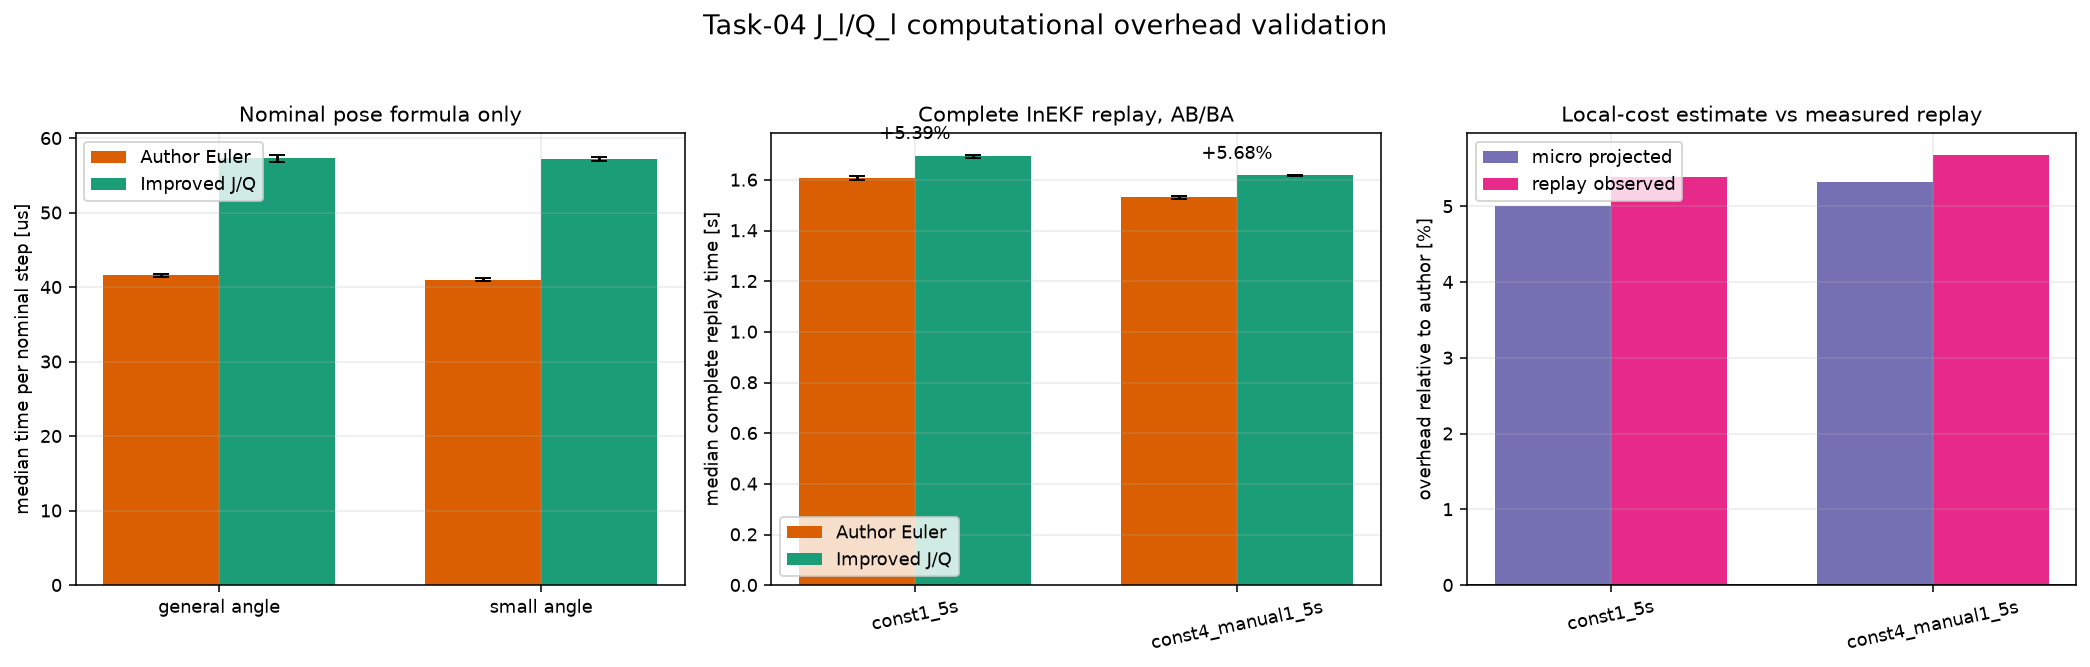
\includegraphics[width=\textwidth]{../imu-uwb-inekf-update-improve/results/task04_compute_overhead/overhead.png}
\caption{局部公式、完整 AB/BA 回放，以及按真实小角比例加权的投影与实测对照。
误差线为 MAD。}
\end{figure}

两组完整回放绝对增加均约 $0.087$ s/5 s 数据，即约
$17$ ms 桌面单核 CPU 时间/秒数据。改进后仍以约 $2.95$--$3.09$ 倍实时速度
回放。8 轮中每一轮改进版均稍慢，最终状态对各自变体逐位确定；事件数、拒绝数和
有限性检查全部通过。

\clearpage
\section{作用量级与总 UWB 50 Hz 评估}

\subsection{为何当前收益近乎为零}

由小角展开
\begin{equation}
\begin{aligned}
J_l(\phi_k)
 &=I+\frac12\Phi_k+\frac16\Phi_k^2+O(\|\phi_k\|^3),\\
Q_l(\phi_k)
 &=\frac12I+\frac16\Phi_k+\frac1{24}\Phi_k^2
   +O(\|\phi_k\|^3),
\qquad
\Phi_k=(\omega_k\Delta t)^\wedge ,
\end{aligned}
\end{equation}
作者式相对精确式漏掉的首项为
\begin{equation}
\boxed{
\delta v_k\approx\frac12R_k(\omega_k\times a_k)\Delta t^2,\qquad
\delta p_k\approx\frac16R_k(\omega_k\times a_k)\Delta t^3.}
\end{equation}
本数据的 IMU 传播间隔中位数约 $0.991$ ms，故速度和位置修正分别受到
$\Delta t^2\sim10^{-6}$ 和 $\Delta t^3\sim10^{-9}$ 的强烈缩小。用原始 IMU
估算，const1 全频回放的单步速度差中位/p95 仅
$0.496/3.051~\mu$m/s，单步位置差中位/p95 仅 $0.158/1.636$ nm。
这些确定性截断项远小于偏置、噪声、UWB 几何和调参误差。

因此，若只考察当前 Python 实现和当前数据，约 $5.4\%$--$5.7\%$ 的完整回放
CPU 代价没有换来工程显著的 RMSE 收益，可以称为``实际精度收益基本可忽略''。
但该修正仍是分段常值 IMU 模型下的正确闭式积分，不能等同于数学上无效，也不能
外推到低 IMU 频率、高角速度或长时间无外部观测的场景。

\subsection{总 TDoA 更新率限制为 50 Hz}

实验先完成原测距对和时长筛选，再在 50 Hz 均匀网格上选择时间最近的原始 TDoA
行并去重，不插值、不合成。const1 从 14,289 次降为 1,501 次，实际
$50.0053$ Hz；const4 从 25,915 次降为 3,001 次，实际 $50.0023$ Hz。
两种传播式仍接收完全相同的数据、初值、协方差和门限。

\begin{table}[H]
\centering
\small
\caption{总 UWB 50 Hz 时，改进式相对作者式的 RMSE 变化}
\begin{tabular}{lrrrr}
\toprule
数据 & 位置 & 速度 & 姿态测地角 & yaw\\
\midrule
const1 前 30 s
 & $+0.000630\%$ & $+0.007372\%$ & $-0.012440\%$ & $-0.014389\%$\\
const4 manual1 前 60 s
 & $-0.004097\%$ & $-0.036448\%$ & $-0.010310\%$ & $-0.010639\%$\\
\bottomrule
\end{tabular}
\end{table}

const1 的位置/速度极微小退化而姿态/yaw 极微小改善，const4 四项极微小改善；
符号不稳定，最大幅度只有 $0.0365\%$。最大位置状态差在 const1/const4 为
$0.164/1.113$ mm，其中 const4 虽高于全频的 $0.497$ mm，却仍未转化为显著
RMSE 收益。作者式和改进式的 UWB 拒绝数分别保持 $0/0$、$12/12$。

\begin{table}[H]
\centering
\small
\caption{作者式中，总 UWB 50 Hz 相对源频率的绝对指标变化}
\begin{tabular}{lrrrr}
\toprule
数据与源频率 & 位置 & 速度 & 姿态测地角 & yaw\\
\midrule
const1，$476.317\to50.005$ Hz
 & $+26.435\%$ & $+38.763\%$ & $-16.672\%$ & $-18.123\%$\\
const4，$431.920\to50.002$ Hz
 & $+9.033\%$ & $-9.006\%$ & $+117.978\%$ & $+136.746\%$\\
\bottomrule
\end{tabular}
\end{table}

UWB 只直接观测位置，速度和姿态经状态相关性间接受影响；原测量含噪，且本实验
没有为 50 Hz 重新调整协方差，所以间接指标不必随频率单调变化。两个数据的位置
RMSE 都明显变差，const4 姿态/yaw 严重变差，说明降频主要削弱了整个滤波器的
外部约束，并没有专门放大这一传播修正。

关键是 UWB 降频并未把 IMU 传播步长从约 1 ms 变为 20 ms。作者联合事件回放中，
50 Hz 时传播 dt 的 p95 反而从约 $1.75$ ms 降为约 $1.09$ ms，时间步更均匀。
若所谓 50 Hz 是每个 TDoA2 测距对的频率，则 8 对合计约 400 Hz，接近本数据的
$431.9$--$476.3$ Hz，应更接近全频结论。只有 IMU 自身降至 50 Hz 时，单步首项
速度/位置修正才会按尺度分别放大约 $20^2=400$ 倍和 $20^3=8000$ 倍；该情形还需
重新处理同步与噪声离散化，不能由本次 UWB-only 降频实验代替。

\begin{figure}[H]
\centering
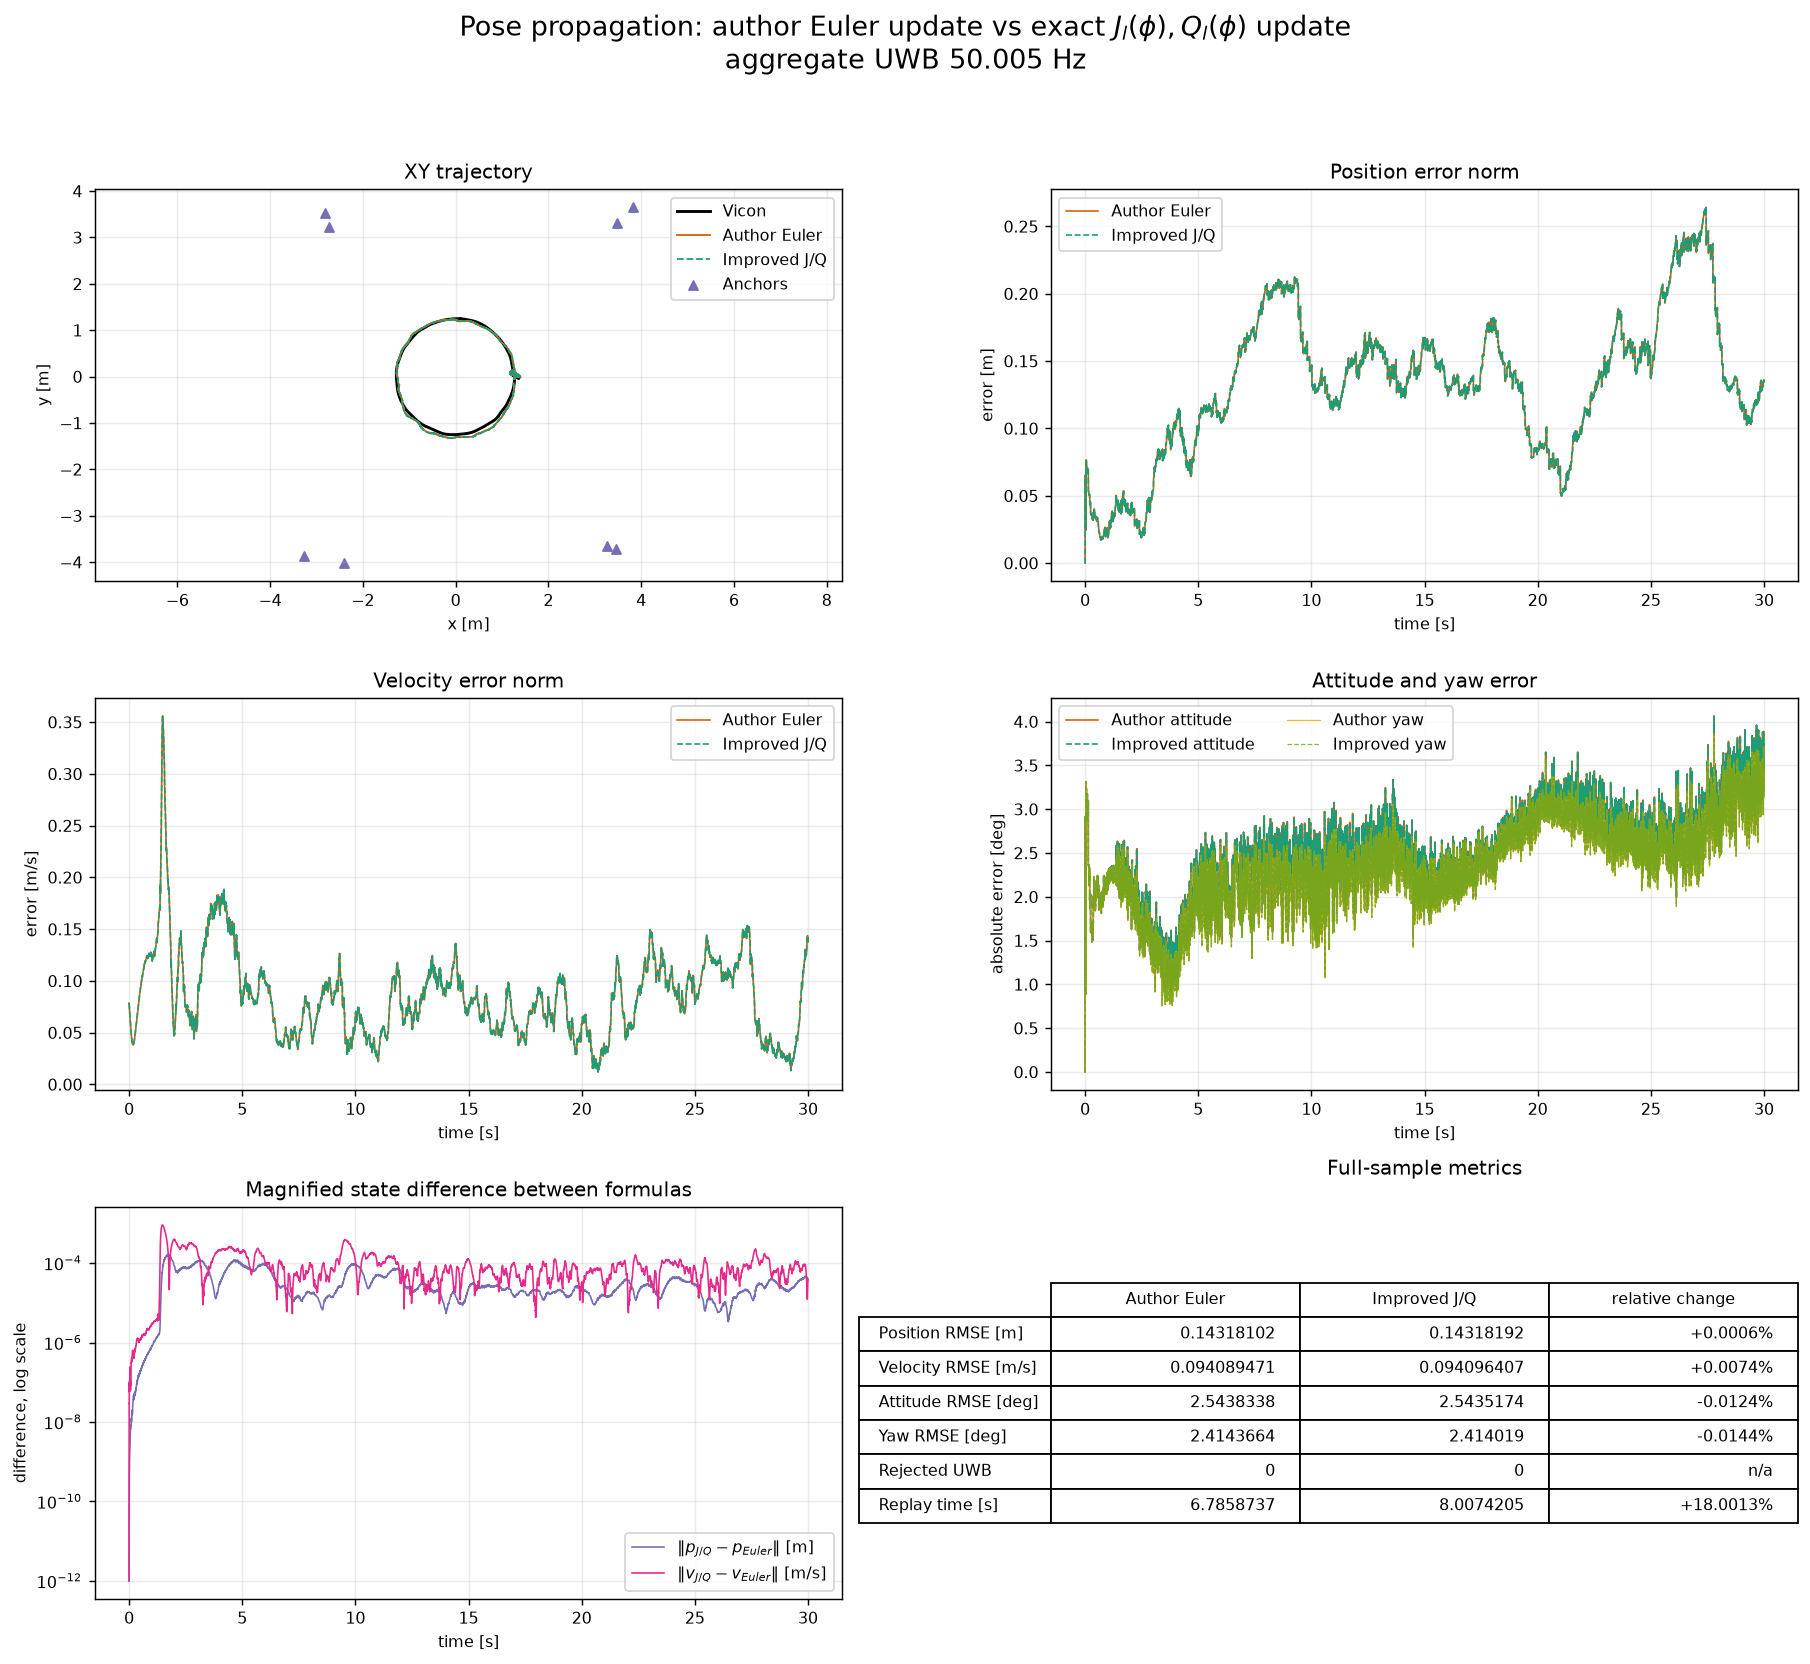
\includegraphics[width=\textwidth]{../imu-uwb-inekf-update-improve/results/task04_const1_30s_uwb50hz/comparison.png}
\caption{const1 总 UWB 50 Hz。轨迹连续，两公式主曲线视觉上重合；放大后的
状态差有限，位置/速度 RMSE 没有因精确积分而改善。}
\end{figure}

\clearpage
\begin{figure}[H]
\centering
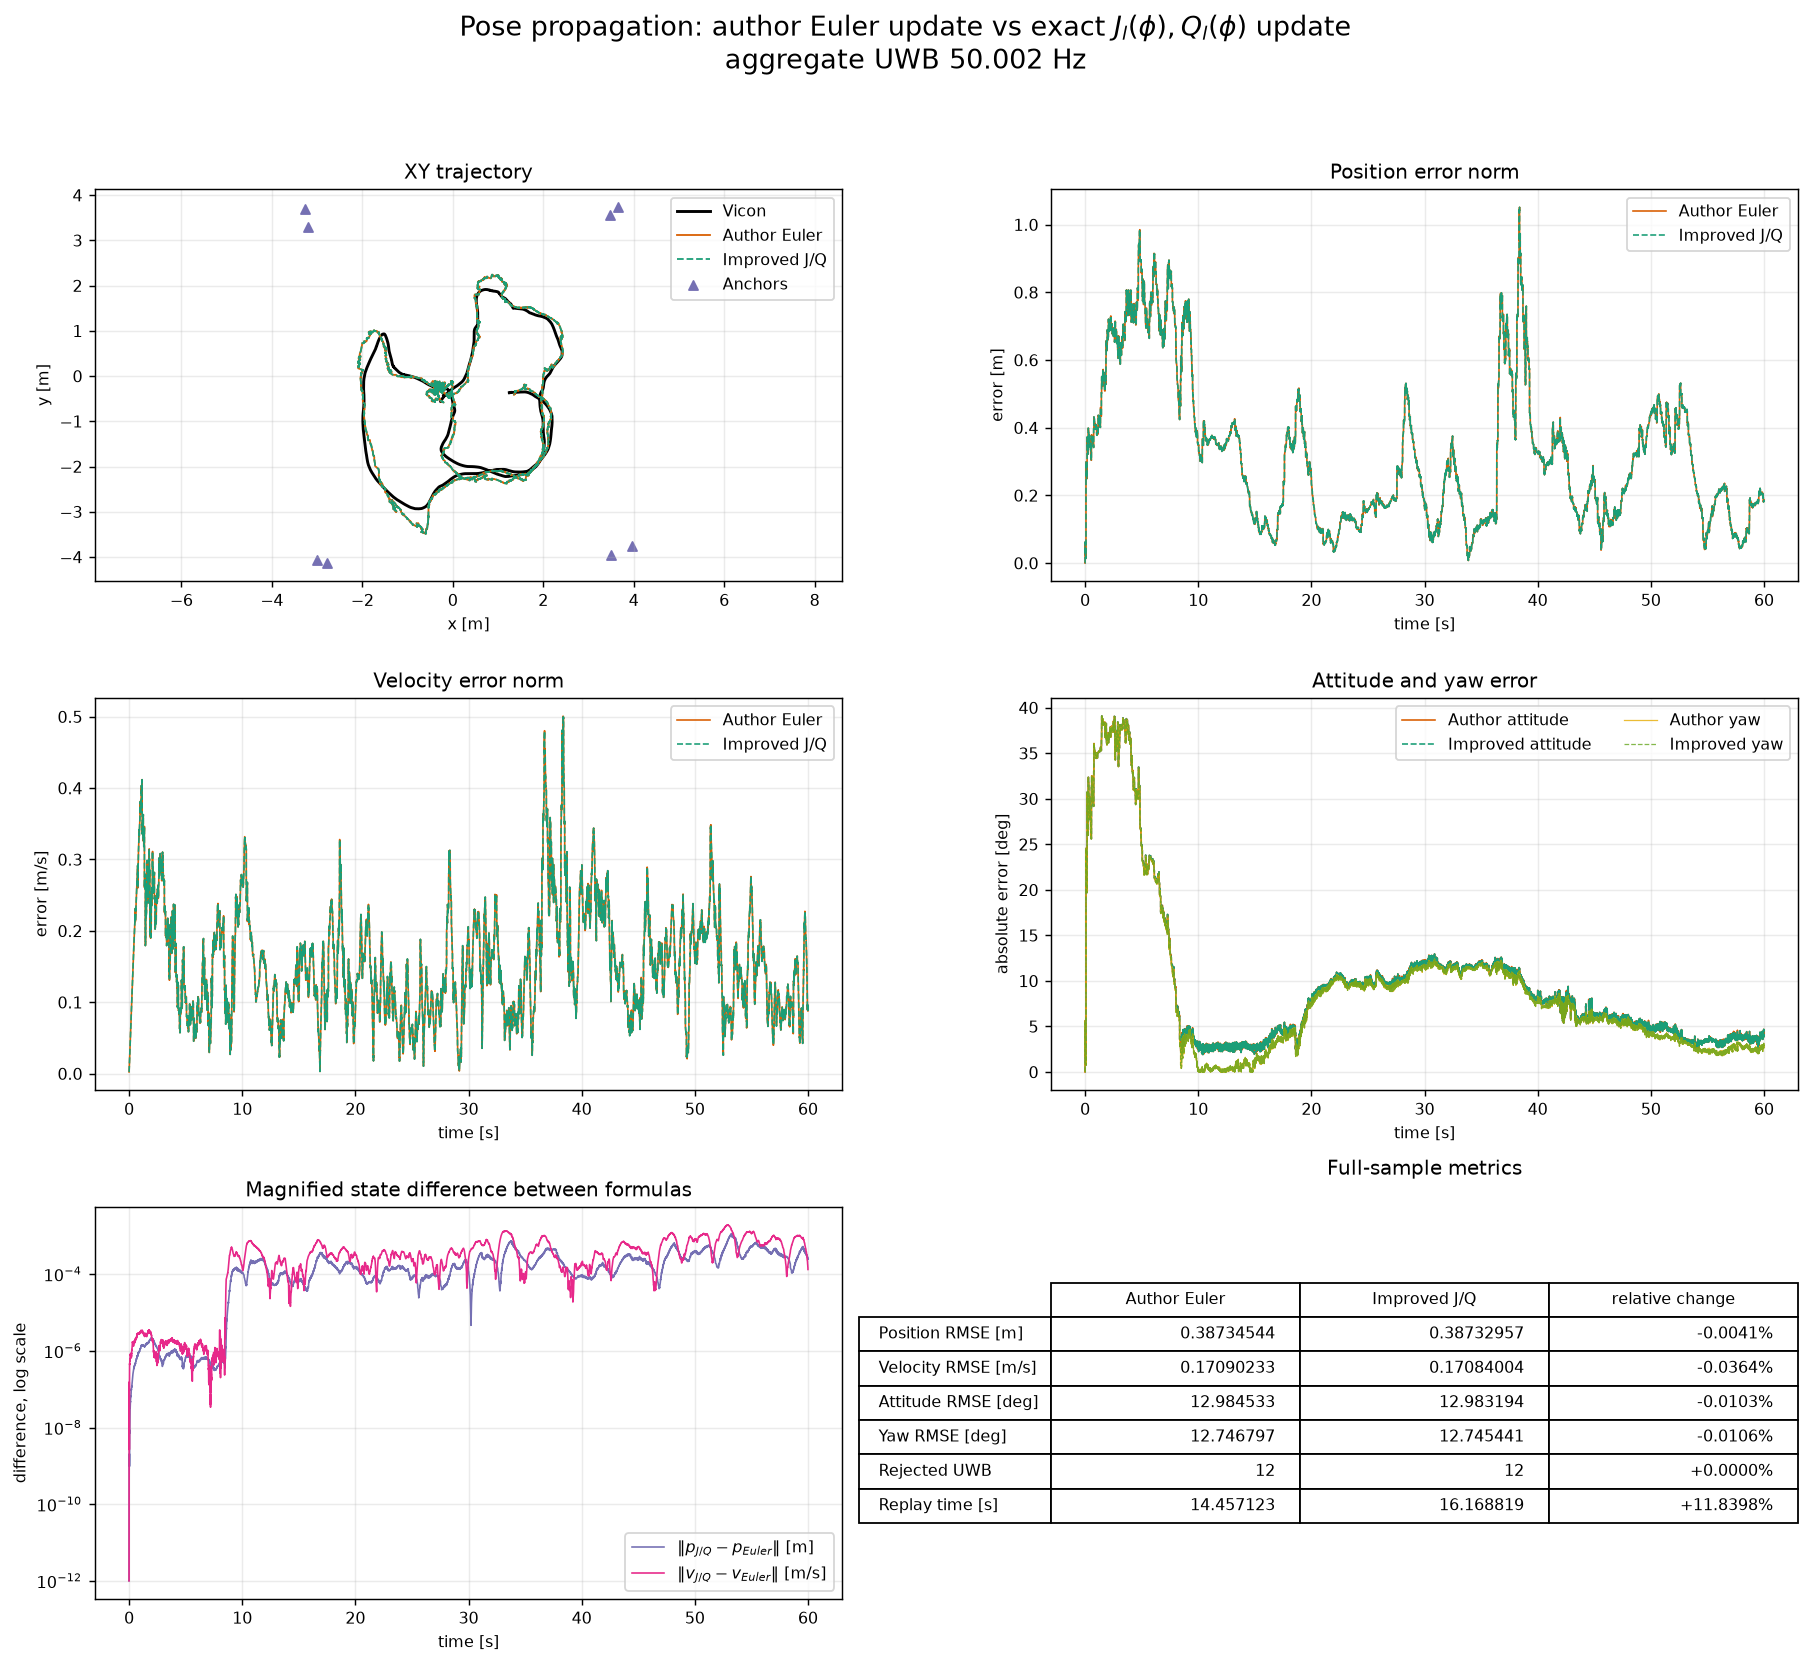
\includegraphics[width=\textwidth]{../imu-uwb-inekf-update-improve/results/task04_const4_manual1_60s_uwb50hz/comparison.png}
\caption{const4 manual1 总 UWB 50 Hz。前约 8 s 的大姿态瞬态同时存在于两种
公式，属于共同滤波行为；没有由改进式新增的跳变或发散。}
\end{figure}

\clearpage
\section{结论与边界}

本任务完成的是分段常值 IMU 模型下的确定性位姿积分精化，不是滤波器其他环节的
重构。两组图片已目视检查：轨迹连续、误差峰值与数据运动一致、无新增发散或异常
跳变，差异放大曲线也没有数值爆炸。开销测试表明当前 Python 实现的局部位姿公式
增加约 $38\%$--$39\%$，但完整 InEKF 只增加约 $5.4\%$--$5.7\%$；该代价在
当前桌面回放中不破坏实时性。

补充的总 UWB 50 Hz 实验进一步表明：降低外部观测频率会改变整体滤波精度，但
不会改变约 1 ms 的 IMU 主传播步长，因此没有稳定放大 $J_l/Q_l$ 的相对收益。
当前条件下最合理的工程判断是保留其``模型正确性修正''定位，同时承认精度收益
基本可忽略；若计算资源严格受限，应在目标机上根据正确性要求与约 $5.5\%$ 的
实测 Python 开销做取舍。

绝对时间依赖 CPU 频率、系统负载和 NumPy/SciPy 版本，不能外推到 MCU、C++、
Numba 或目标机 WCET。若后续单独授权做等价计算优化，可研究
$R(Ja)$ 的乘法结合顺序和三角函数复用；本轮没有修改核心算法，也没有把潜在收益
冒充实测结果。

运行入口为
\texttt{imu-uwb-inekf-update-improve/run\_task04.ps1}；默认
\texttt{-Mode quick} 先执行自动测试，再回放 const1 前 30 s 并生成 PNG、JSON
和 CSV；\texttt{-Mode overhead} 执行本节基准。完整说明见同目录
\texttt{TASK04\_README.md}。

\end{document}
